\clearpage %%% für Druck

\subsubsection{Scrum}
\label{sec:Kap-2.2.3.2}

\sttpLeserfuehrung{Bilder/Kapitel-2/Leserfuehrung/vorgehensmodelle_agile_illustration.pdf}{Bilder/Kapitel-2/Leserfuehrung/vorgehensmodelle_scrum.pdf}

Scrum ist ursprünglich für Managementprozesse in der Automobilindustrieproduktion entwickelt worden. Ken Schwaber und Jeff Sutherland  stellten es Mitte der 1990er Jahre erstmals für die Verwendung in der Softwareentwicklung vor. Zunächst war Scrum nur ein leichtgewichtiges Modell unter einigen anderen leichtgewichtigen Modellen. Seit Mitte der 2000er Jahre erhielt Scrum dann im breiten Bewusstsein immer mehr die Rolle als wichtigstes agiles Vorgehensmodell. Das hat vermutlich auch damit zu tun, dass man sich seit 2002 offiziell als Scrum Master (eine Rolle im Scrum Team) zertifizieren lassen kann. 

Scrum ist für kleine Teams mit üblicherweise weniger als 10 Personen \cite[5]{sch20} vorgesehen, für größere Projekte können mehrere Scrum-Teams gebildet werden. Scrum berücksichtigt deutlich stärker als XP die Projektmanagementsicht, indem es einen strikten organisatorischen Rahmen mit festen Kommunikationsformaten, Rollenzuständigkeiten und Kontrollmöglichkeiten des Projektfortschritts vorgibt. In Bezug auf konkrete Entwicklungsmethoden ist Scrum dagegen sehr viel flexibler als XP. Die Philosophie hinter Scrum lautet, dass das Entwicklungsteam selbstständig entscheidet, welche Entwicklungsmethoden und -werkzeuge es zur Erreichung seiner Ziele einsetzt. Eine Verbindung von Scrum mit XP-Methoden ist daher sehr gut möglich. 

\minisec{Struktur des Softwareentwicklungsprozesses}
Im  Vergleich mit XP verschwimmen bei Scrum die Grenzen zwischen iterativer und klassisch inkrementeller Entwicklung noch stärker. Während bei XP ein ausgeliefertes Inkrement (Release) in mehreren Iterationen entsteht, wird bei Scrum in jeder Iteration (in Scrum \textit{Sprint} genannt) \marginline{Sprint, Release}
eine lauffähige und (potenziell) vom Kunden einsetzbare Produktversion (ebenfalls \textit{Release} genannt) erzeugt, wobei bereits implementierte Funktionalität in folgenden Sprints wieder überarbeitet werden kann. Ein Sprint in Scrum sollte maximal einen Monat lang sein, in der Praxis üblich ist auch ein Zwei-Wochen-Rhythmus \cite[104]{kom17}. Die Sprint-Dauer für ein Projekt legt das Entwicklungsteam in Absprache mit dem Kunden fest. Wichtig ist dabei, dass alle Sprints des Entwicklungsprojekts gleich lang sein sollen und es somit nicht wie bei XP variable Zeitspannen für eine Iteration gibt. 

Scrum unterscheidet neben dem Entwicklungsteam nur die Rollen 
\marginline{Scrum Master}
\textit{Scrum Master} und Product Owner (s.u.). Der Scrum Master ist dafür zuständig, dass der Scrum-Prozess (insbesondere die vorgegebenen Kommunikations- und Kontrollformate) eingehalten wird. Zudem ist es seine Aufgabe, das Entwicklungsteam von äußeren Einflüssen (\zb Wünsche anderer Projekte oder der Managementebene der Firma) \mbox{abzuschirmen}, sodass das Team in seiner Produktivität nicht unnötig beeinträchtigt wird. Scrum kennt explizit keine Hierarchien im Scrum-Team. So soll insbesondere der Scrum Master nicht mit einem Entwicklungsleiter gleichgesetzt werden. Scrum schließt nicht aus, dass außerhalb der drei genannten Rollen noch weitere Personen am Entwicklungsprojekt beteiligt sein können, wie zum Beispiel Domänenexperten oder externe Berater. Diese gehören dann aber streng genommen nicht zum Scrum-Team.

Scrum  definiert vier feste Kommunikationsformate, die in jedem Sprint zwingend einzuhalten sind: Das Daily Scrum, das Sprint Planning und das Sprint Review (s.u.) sowie die Retrospektive. Das maximal 15-minütige \textit{Daily Scrum} \marginline{Daily Scrum} 
findet jeden Tag zur gleichen Zeit und am gleichen Ort statt. Dabei handelt es sich um ein Treffen des gesamten Teams, das im Stehen ausgeführt wird – eine Maßnahme, die helfen soll die veranschlagte Zeit einzuhalten – und in dem jedes Teammitglied die anderen über den aktuellen Stand seiner Arbeit, die Arbeitsplanung für den kommenden Tag und aufgetretene Probleme informiert. Auf diese Weise kann das Entwicklungsteam täglich seinen Projektfortschritt im Blick behalten.

Die Sprint \textit{Retrospektive} \marginline{Retrospektive}
findet am Ende eines Sprints statt. Die Retrospektive soll für das Scrum-Team die Gelegenheit bieten, „Wege zur Steigerung von Qualität und Effektivität zu planen.“ \cite[10]{sch20}. Hier geht es neben inhaltlichen und organisatorischen Aspekten der Prozessverbesserung vor allem auch um arbeitsatmosphärische (Un)Zufriedenheiten im vergangenen Sprint.

\vspace{-\baselineskip} %%% für Druck

\begin{figure}[h!]
	\centering
	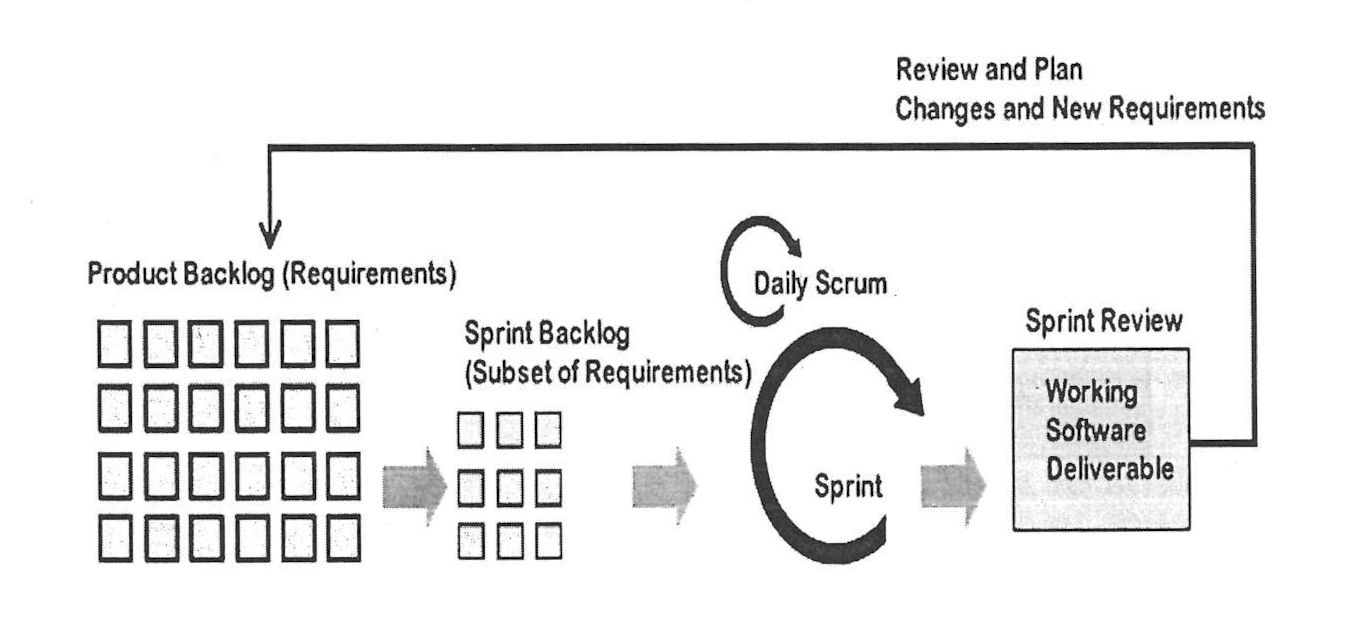
\includegraphics[scale=0.7]{Bilder/Kapitel-2/ScrumProzess.png}
	\caption[Der Scrum-Prozess]{Der Scrum-Prozess \cite[7312]{gut15}}
	\label{fig:scrum_prozess}
\end{figure}

\minisec{Einbezug des Kunden}

Die \textit{Product Owner}-Rolle \marginline{Product Owner}
bei Scrum entspricht im Prinzip der Rolle des Kunden\-vertreters bei XP. Sofern mehrere Kundenvertreter ins Entwicklungsprojekt einbezogen sind, übernimmt einer von ihnen die Product Owner-Rolle. Der Product \mbox{Owner} spezifiziert und priorisiert die Anforderungen an das zu entwickelnde Software\-produkt sowie die zugehörigen Akzeptanztests.

\minisec{Umgang mit Anforderungen}

An Artefakten definiert Scrum neben dem Release nur das sogenannte 
\marginline{Product Backlog, Sprint Backlog}
\textit{Product Backlog} und das \textit{Sprint Backlog}. Das Product Backlog enthält die Anforderungen an das zu erstellende Softwareprodukt. Es wird vom Product Owner erstellt und kontinuierlich ergänzt, verändert und verfeinert, wobei der Product Owner gegebenenfalls von weiteren Domänenexperten oder vom Entwicklungsteam unterstützt wird. Die Verantwortung für das Product Backlog und die Priorisierung der darin enthaltenen Anforderungen (Product Backlog Items genannt) liegt immer beim Product Owner. Über das Product Backlog kann der Product Owner neue Anforderungen jederzeit einbringen, bestehende streichen oder verändern und somit im gesamten Verlauf des Entwicklungsprojekts flexibel Einfluss auf die Entwicklungsrichtung nehmen. 

Das Sprint Backlog enthält diejenigen Anforderungen des Product Backlog, die im aktuellen Sprint umgesetzt werden sollen. Spätestens wenn ein Backlog Item (eine definierte Anforderung) des Product Backlog in das Sprint Backlog aufgenommen wird, müssen Product Owner und Entwicklungsteam eine sogenannte \marginline{Definition of Done}
\textit{Definition of Done (DoD)}  
%\sttpkapitelverweis{Definition of Done}{Kap.~\ref{sec:Kap-x.y}}
für dieses Item erstellen. Eine DoD legt fest, welche Merkmale die Umsetzung einer Anforderung aufweisen muss, damit die Umsetzung als „fertig“ (heißt auslieferbar) gilt. Scrum macht keinerlei Vorgaben, wie eine DoD aussehen muss. Möglich wäre es zum Beispiel, die Erfüllung von bestimmten Akzeptanztests als Kriterium einer DoD anzusetzen.

Zu Beginn jedes Sprints legen Entwicklungsteam und Product Owner im 
\marginline{Sprint Planning} 
\textit{Sprint Planning} gemeinsam fest, welche der vom Product Owner mit höchster Priorität versehenen Product Backlog Items umgesetzt werden können. Spätestens dann müssen die einzelnen Items so detailliert spezifiziert sein (unter anderem durch die DoD), dass eine Aufwandsschätzung möglich ist. Es ist Aufgabe des Scrum Masters während des Sprints diese Aufwandsschätzung kontinuierlich mit dem real geleisteten Aufwand abzugleichen und zu kontrollieren, ob das Sprint-Ziel erreicht werden kann. Unter Umständen muss das Team in Absprache mit dem Product Owner den Leistungsumfang des Sprints reduzieren, indem bestimmte vorgesehene Items nicht umgesetzt werden. Ansonsten sind während eines Sprints keine Änderungen erlaubt. Auch neue Anforderungen, denen der Product Owner eine höhere Priorität zuteilt als den aktuell in der Umsetzung befindlichen, müssen bis zum nächsten Sprint warten, ein Tausch von Items ist nicht möglich. 

Dieses Einfrieren von Anforderungen während eines Sprints ist Scrums Lösung für den Spagat zwischen der Möglichkeit von Anforderungsänderungen und der Notwendigkeit von Planungssicherheit. Für Bertrand Meyer, der für sein 2014 erschienenes Buch „Agile! The Good, the Hype and the Ugly“ \cite{mey14} verschiedene agile Mo\-delle und Methoden analysiert hat, ist diese Scrum-Lösung die bedeutendste Idee des agilen Umfelds.

\vspace{3mm} %%% für Druck

\sttpzitat{„If out of my long immersion in agile methods for the preparation of this book I had to retain just one idea, that would be it. The principle is innovative, applicable, and effective.“ \cite[140]{mey14}}{Betrand Meyer über das Einfrieren von Anforderungen während eines Sprints}

\vspace{3mm} %%% für Druck

Im Kommunikationsformat des \textit{Sprint Review} \marginline{Sprint Review} begutachten und diskutieren Entwicklungsteam, Product Owner und eventuelle weitere Domänenexperten die Ergebnisse des Sprints (Umsetzung der Anforderungen). Daraus resultierende notwendige Änderungen oder neue Anforderungen werden ins Product Backlog eingetragen.

\minisec{Einordnung von Scrum}

Die von Scrum vorgegebenen Elemente sind fast ausschließlich auf der organisatorischen Ebene des Softwarenentwicklungsprojekts angesiedelt. Mit welchen Techniken die Ziele des Sprints erfüllt werden, wie die Aufgabenverteilung im Team aussieht, aber auch, in welcher Art und Weise die vorgegebenen Kommunikationsformate ausgestaltet werden, bleibt dem konkreten Team überlassen. Dieses ist damit in höchstem Maße (im positiven wie im negativen Sinne) eigenverantwortlich. In der Praxis werden insbesondere Teammitglieder, die schon in Scrum-Projekten gearbeitet haben, Ideen zu Prozessabläufen, Entwicklungsmethoden und -werkzeugen beisteuern können.

Wie für XP gilt auch für Scrum, dass es sich erst dann um einen Scrum-Prozess handelt, wenn \textbf{alle} Scrum-Regeln eingehalten werden. Nichtsdestotrotz lassen sich einzelne Scrum-Elemente auch in anderen Modellen verwenden. 

Im Gegensatz zu anderen agilen Modellen gibt es gegenüber Scrum wenige kritische Stimmen. Das hat sicher damit zu tun, dass Scrum keinerlei Vorgaben zu Entwicklungsmethoden macht und insofern, auch im Vergleich zu XP, deutlich weniger radikal wirkt. Theoretisch wäre es sogar möglich, innerhalb eines Sprints in einem wasserfallartigen Vorgehen zu arbeiten oder die einzelnen Product Backlog Items so detailliert schriftlich zu fixieren, dass eine umfassende Dokumentation der Anforderungen inklusive getroffener Entwurfsentscheidungen entsteht. In der Regel wird Scrum aber in Kombination mit agilen Methoden wie Test-First Development und Continuous Integration eingesetzt. Die Herausforderungen bezüglich der Vertragsgestaltung für Auftragsarbeiten und bezüglich vorhandener Unternehmensstrukturen (\zb Controllingabläufe, Berichtspflichten), die auf sequentielle Modelle ausgerichtet sind, teilt Scrum mit anderen agilen Modellen. 